\chapter[Toy models of athermal deformation]{Toy models \\ of athermal deformation\label{ch:ToyModels}}

Simulations of athermal deformation of Lennard-Jones systems are expected to give insight about the behavior of slowly oscillatory sheared particle systems. Understanding the phenomenology observed in such simulations, however, appears as a daunting task. The main difficulty arises from the complicated AQS dynamics in a highly dimensional configuration space.
A fruitful strategy to get a clearer idea of what are mechanisms that lead to the transition observed at $\gamma_{c}$ in \autoref{ch:ParticleModelsResults} is the development of toy models. These should be more easily tractable and understandable (ideally analytically solvable), but still show the key phenomenology observed in the Lennard-Jones simulations. In this chapter, for this scope, we describe and employ two models: the NK model \cite{isner2006generic}, which we describe in \autoref{sec:NKModel}, and the TM (transition matrix) model, a novel representation that treats AQS deformation cycles as transition matrices and is described in \autoref{sec:TransitionMatrixModel}. 
With the aid of such toy models, the essential ingredients needed to observe the same phenomenology seen in the Lennard-Jones simulations can be identified. One example of common behavior observed in all these systems (LJ, NK and TM models) is the capability to retain a memory of their history, similarly to what is observed in the noncolloidal suspensions in \cite{keim2011generic}. We will deal with this subject separately, in \autoref{ch:Memory}.

\section{NK model \label{sec:NKModel}}

In this section we review the so-called NK model mentioned in \autoref{ch:Introduction} and used in \cite{isner2006generic} to get insights about rejuvenation and overaging in glasses\footnote{The only difference between our version of the NK model and that in \cite{isner2006generic} is the addition of the constraint of constant sum of the values of the spins.}. This model takes its name from the two main parameters in it. In what follows, we perform (whenever possible) on it measurements that are equivalent to those performed on the LJ system in \autoref{ch:ParticleModelsResults}. In this sense we extend the work in \cite{isner2006generic} on the NK model to multiple driving cycles, in the same way as \autoref{ch:ParticleModelsResults} extends the study in \cite{lacks2004energy} on LJ systems.

\subsection{Features of the NK model}

The NK model is constructed on a lattice of $N$ (even) lattice sites occupied by ``spins'' $m_{i}$ that can take either the values $0$ or $1$.
\begin{equation}
\{m_1, m_2, \ldots, m_i, \ldots, m_{N} \} \in \{0, 1\}^{N}
\end{equation}
Furthermore, we limit (for reasons clarified in \autoref{app:NKDetails}) the space of allowed configurations to those that satisfy the constraint
\begin{equation}
\sum_{i} m_{i} = \frac{N}{2}
\end{equation}
(this is equivalent to taking the set of states of constant magnetization $N/2$ in the Ising model).
There are $\binom{N}{N/2}$ such configurations. From a geometrical point of view these configurations are the $N$-tuples that identify the coordinates of the vertices which define a $N$-dimensional unit hypercube and that lie on the $\sum_{i} m_{i} = N/2$ hyperplane.\\ 
In addition, we introduce:
\begin{itemize}
	\item an ordered list of $K$ ``neighbors'' for each $i$-th spin, specified by the map $J$: 
	\begin{equation}
		m_{i} \xrightarrow{J} \{m_{i}^{1}, \ldots, m_{i}^{K}\}
		\label{eq:NKNeighbors}	
	\end{equation} 
	The choice of the list of neighbors for a given spin is random.
	\item two functions $a$ and $b$ connecting the set $\{0, 1\}^{K+1}$ (the set of all the $(K+1)$-tuples formed by ones and zeros) to the intervals $[-1,1]$ and $[0,1]$ respectively
	\begin{align}
		\{0, 1\}^{K+1} & \xrightarrow{a} [-1,1]  & \quad		\{0, 1\}^{K+1} & \xrightarrow{b} [0,1]
		\label{eq:NKCouplings}
	\end{align}
	The correspondence between a given $(K+1)$-tuple and the numerical value is chosen randomly with a uniform probability within the respective intervals.
\end{itemize}
 
The energy of the system depends on the values of the spins, $E = E(m_{1}, \ldots, m_{N})$ according to
\begin{equation}
	E = -\frac{1}{2} \sum_{i = 1}^{N} \left[ 1 + \sin(2 \pi (a_{i} + \gamma b_{i})) \right]
	\label{eq:NKEnergy}
\end{equation}
where $\gamma$ is a parameter that can be varied continuously.

In addition, we define two NK configurations as adjacent if one is turned into the other by swapping the values at two sites $i$ and $j$ such that $m_{i} \neq m_{j}$. Said in geometrical terms, two configurations are adjacent if they represent two vertices that lie at the extremes of a diagonal of a face of the $N$-dimensional unit hypercube. Each configuration has thus $N^{2}/4$ configurations that are adjacent to it.

\subsection{Energy landscape of the NK model}

The NK model is known to possess a discrete energy landscape whose roughness (a measure of which is given by the number of local minima in the landscape) is tuned by the value of the parameter $K$. The landscape is smooth for $K = 0$ and the roughness is increased as $K$ is increased. To see this consider the case $\gamma = 0$ for simplicity. If $K=0$, when performing the sum in \autoref{eq:NKEnergy} one sums contributions that are simply $1 + \sin(2 \pi a_{i})$, where $a_{i}$ can assume only two values in the interval $[-1,1]$, depending solely on whether $m_{i} = 1 $ or $0$, as no spin has neighbors. It's clear that the energy increases or decreases monotonically with the ``magnetization'' $\sum_{i} m_{i}$. As in our case such quantity is fixed, all the allowed configurations have the same $E$. This implies that by moving from a given configuration to any adjacent one the energy can't change and the landscape is thus \emph{flat}. In the case $K = N-1$ each spin is a neighbor of any other. To estimate the roughness of the landscape, we compare the energies of two adjacent structures, that differ by the swapping of two spins. Each term in \autoref{eq:NKEnergy} is affected by such a swap, and so all the $a_{i}$'s that contribute to the energy of the two configurations differ. Being the $a_{i}$'s random and uncorrelated, there won't be correlation between the energies of two adjacent configurations. Consequently, the structure of the overall landscape will be rough. 

While $K$ is able to tune the roughness of the landscape, the parameter $\gamma$ is able to change continuously the values of the energy of the configurations (and thus the overall landscape). This is similar to what happens in a Lennard-Jones system, in which a macroscopic strain is externally imposed. For this reason, with a slight abuse of terminology, $\gamma$ will be called ``shear strain'' also in the context of the NK model in what follows.

A graph representation of the landscape for low values of $N$ and $K$ is given in \autoref{fig:NKGraph}. Nodes represent single configurations, and edges connect adjacent configurations. 
\begin{figure}
\centering 
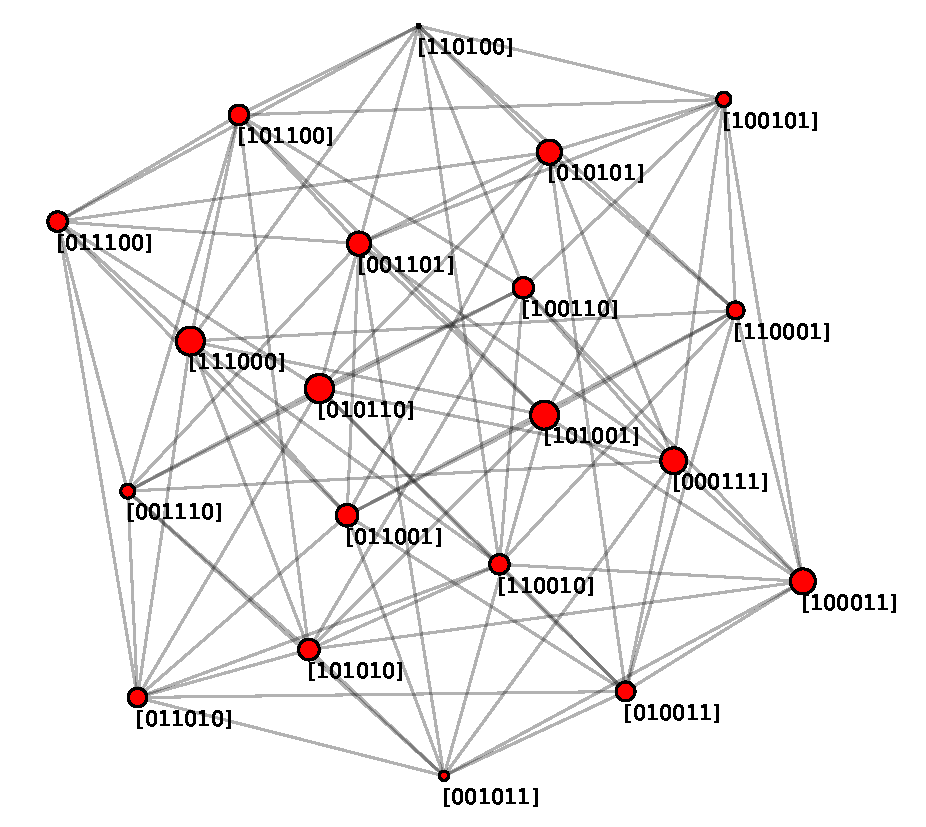
\includegraphics[width=0.6\textwidth]{NKGraph.pdf} 
\caption{Graph representation of the space of configurations of the NK model with $N=6$. In this case, only 20 configurations are allowed. Edges in the graph connect adjacent configurations, and the size of the node denotes the value of $E$ (in arbitrary units), with bigger nodes indicating a lower energy. As $\gamma$ in \autoref{eq:NKEnergy} is changed, one can imagine that the sizes of the nodes vary accordingly. Following the steepest descent (SD) starting from a given node, in this case, means moving from node to node by choosing the largest node accessible via an edge at each step.\label{fig:NKGraph}}
\end{figure}
To summarize, the NK model is similar to the LJ model because it possesses a rugged energy landscape which is deformable by varying the parameter $\gamma$, and concepts and protocols that apply for the latter can be transferred to the former.
For instance, starting from an initial configuration, energy can be minimized by a steepest descent (SD) procedure. A SD in the NK energy landscape consists in moving from a configuration to the adjacent one with the lowest $E$, and iterating this procedure until when no move to an adjacent configuration results in a decrease in $E$. Using such a protocol, any configuration can be mapped onto a local minimum, i.e. an inherent structure of the NK landscape. This fact, together with the dependence on $\gamma$ of the landscape, allows to define an athermal quasi static ``deformation'' procedure on NK systems too. The procedure follows closely that described in \autoref{sec:LJDeformation}:
\begin{enumerate}
	\item Take an inherent structure of the NK landscape. This can be obtained by any configuration by means of the SD algorithm.
	\item Increment the value of $\gamma$ in \autoref{eq:NKEnergy} by a small amount $d\gamma$. As in the LJ case, the value of $d\gamma$ should be small enough so that the modification of the landscape is slow enough and no displacements to adjacent inherent structures are ``missed''\footnote{In other words, $d\gamma$ should be small enough that if a smaller $d\gamma'$ was employed it would yield exactly the same evolution.} by the AQS dynamics.
	\item Apply the SD procedure to the configuration.
\end{enumerate}

As AQS can be applied to the NK model, it's interesting to check whether the same phenomenology seen in AQS deformation of Lennard-Jones systems can be observed in it. However, one should be aware that the two models still bear differences:

\begin{itemize}
	\item The NK model has a \emph{discrete} configuration space. This makes the AQS dynamics of NK systems somewhat different to that of LJ systems. In the NK case, the system occupies one given point of the available configuration space as $\gamma$ is changed, and stays there until it ``jumps'' to another inherent configuration as soon as the initial point is not an inherent configuration anymore. In the LJ case, instead, systems do \emph{always move} in the configuration space as $\gamma$ is varied (as described in \autoref{sec:LJDeformation}).
	\item Due to the discrete nature of the landscape, minimization is trickier in the NK case. While in the LJ case \emph{local} quantities (e.g. the calculation of a potential energy gradient) allow to determine the direction to follow to reach an inherent structure, in the NK model \emph{all} the energies of adjacent configurations need to be calculated in order to choose the adjacent configuration with the lowest energy (if there is one). This operation requires $O(N^{2})$ energy calculations to be performed (as the number of adjacent configurations scales with $N^{2}$, see above) and is thus computationally unfeasible for large values of $N$. More details about the complexity of the minimization in the NK space are reported in \autoref{app:NKDetails}.
	\item While the LJ energy landscapes depend on the values of the $\epsilon$ and $\sigma$ parameters in \autoref{eq:BinaryLennardJonesPotential} and the boundary conditions of the simulation boxes, the definition of the landscape in the NK case requires the introduction of a much larger number of parameters. This is because the lists of neighbors specified by $J$ can be realized in many different ways\footnote{The number of ways in which $J$ can be chosen is related to the number of possible ``friendship networks'' in a group of $N$ people if everyone has $K$ friends and ``friendship'' is a symmetric relation (so that if $A$ is a friend of $B$ then $B$ is a friend of $A$). In more formal terms, this is also related to the number of \emph{regular graphs} having degree $K$ (as in the the NK model each spin has $K$ other spins coupled to it) and $N$ vertices. Actually this number cannot be expressed in a closed form (only asymptotic results exist in the literature)!}, and $a$ and $b$ in \autoref{eq:NKNeighbors} and \autoref{eq:NKCouplings} require $2^{K}$ values each to be defined.
\end{itemize}

Having noted this, we can study the NK model under athermal quasi-static deformation, and compare the results with what is obtained with the LJ model. Such comparison is meaningful, because the two systems share important features. At the same time it's not trivial, becuase, as explained above, the two models are ``sufficiently different'' so that a common qualitative behavior can't be taken for granted a priori.

\section{Transition matrix (TM) model \label{sec:TransitionMatrixModel}}

Both the LJ and NK models possess a rugged landscape that is modified during the deformation. The behavior under oscillatory deformation, in particular, thus depends on the detailed features of the landscape.
Would it be possible to predict the behavior of such models qualitatively, without encoding in detail the features of the energy landscape, but using a sort of ``high-level'', abstract description of its evolution? This is what the ``transition matrix'' method (TM) aims to do, by exploiting some of the ideas already outlined in \autoref{sec:LJDeformation}. A nice feature of it is that it provides a description that can be applied both to the LJ and NK models.\\

The starting point of the TM approach is to look at a cycle of AQS deformation from a mere ``mathematical'' point of view.
In that perspective, an AQS cycle is a correspondence between the set of $M$ inherent structures of the energy landscape at $\gamma = 0$ into itself\footnote{In more mathematical terms, an AQS cycle defines an \emph{endomorphism} of the set of inherent structures of the landscape such that $\gamma = 0$.}. This is because a valid starting configuration is an inherent structure of the $\gamma = 0$ landscape, and it is transformed into another inherent structure of the same landscape at the end of the deformation cycle. Each of these inherent structures can be identified by an index $i$, and associated to a $M$-dimensional vector $\mathbf{R_{i}}$ whose components are all zero but for the $i$-th one, which is set equal to 1. Then, they can be taken as starting points of a deformation experiment where a single AQS cycle is performed and the inherent structure reached at the end is recorded.
This allows to construct a \emph{transition matrix} $P$, such that
\begin{equation}
	P \mathbf{R_{i}} = \mathbf{R_{f}}
	\label{eq:TransitionMatrixCycle}
\end{equation}
where $\mathbf{R_{i}}$ and $\mathbf{R_{f}}$ are the vectors associated to the initial and final inherent states.
Here we list some of the properties of the $P$ matrix, which descend directly from the features of AQS dynamics:
\begin{itemize}
	\item $P$ encodes the entire information about the evolution of any inherent structure under cyclic deformation, as by using \autoref{eq:TransitionMatrixCycle} one can determine the final inherent structure $\mathbf{R_{f}}$ given any intial one $\mathbf{R_{i}}$.
	\item $P$ is a sparse $M \times M$ matrix, and $P_{ij} = 1$ if and only if the state associated to $\mathbf{R_{j}}$ is mapped onto the inherent structure $\mathbf{R_{i}}$ in the AQS cycle. The consequence is that all the columns have exactly one non-zero entry (equal to one) because each $\mathbf{R_{j}}$ configuration is sent to some other $\mathbf{R_{i}}$ inherent structure by the AQS cycle.
	\item $P$ depends on the value of $\gamma_{max}$, i.e. on the amplitude of the deformation. For very small amplitudes, a sizable fraction of the inherent structures will be unchanged under the deformation, because an AQS cycle will not be effective at destabilizing the starting inherent structures. In this case a given structure will often map onto itself through $P$ and thus $P$ will be very close to the diagonal unit matrix. In general this won't be any longer true for higher values of $\gamma_{max}$.
	\item The determinant of $P$ is, in general, zero. In general, more than one structure will map onto the same final state $\mathbf{R_{f}}$, so that in that case $P$ will define a non-injective function. As the domain of $P$ is also its codomain, $P$ is not surjective, so that there will be structures that are not arrival configurations for any inherent structure (this is illustrated in \autoref{fig:AQSCycleAsMap}). This has the consequence that some rows of the $P$ matrix, in general, are identically zero, and so is the value of $\det P$.
	
	\begin{figure}
	\centering 
	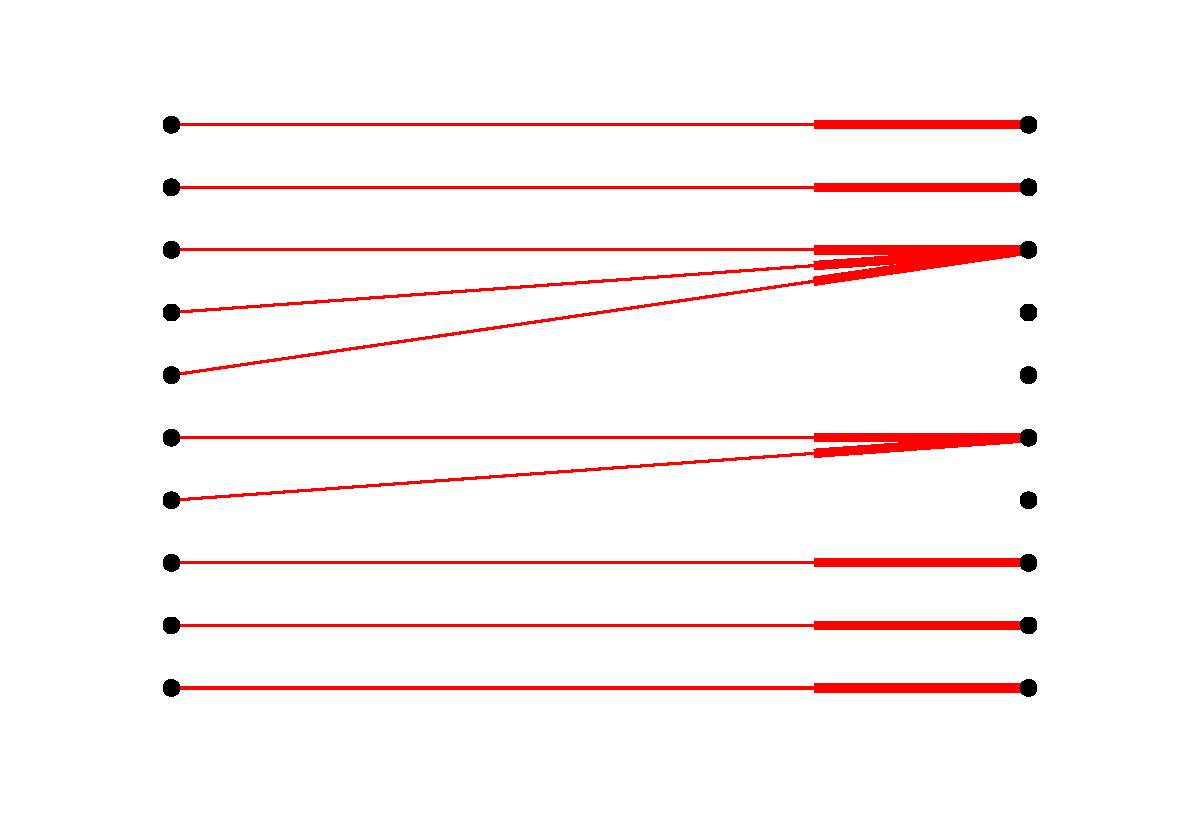
\includegraphics[width=0.5\textwidth]{AQSMap.pdf} 
	\caption{Graph representation of an AQS cycle, that has the effect of mapping the set of inherent structures of the $\gamma = 0$ landscape onto itself. If the application is not injective, it can't be surjective either.\label{fig:AQSCycleAsMap}}
	\end{figure}
	
	\item $M$, in general, is a large number. The size of $P$ is equal to the number of inherent structures of the landscape, and this number, for typical LJ and NK landscapes, is large (exponential in $N$ in the first case, and equal to $\binom{N}{N/2}$ in the second).
	\item The result of a deformation experiment where $L$ cycles (rather than just one) are applied to a given starting configuration $\mathbf{R_{i}}$ is obtained by applying \autoref{eq:TransitionMatrixCycle} repeatedly:
	\begin{equation}
		P^{L} \mathbf{R_{i}} = \mathbf{R_{f}} \qquad \text{where } P^{L} = \underbrace{P \cdot \ldots \cdot P}_{L\text{ times}}
	\end{equation} 
\end{itemize}

\subsection{Classification of states by their transformation properties \label{sec:TMStateClassification}}

A given configuration $\mathbf{R_{i}}$ can transform under the effect of $P$ in different ways:
\begin{enumerate}
	\item \label{it:AbsorbingState} $P \mathbf{R_{i}} = \mathbf{R_{i}}$: in this case $P$ has no effect on $\mathbf{R_{i}}$, so that $\mathbf{R_{i}}$ is an eigenvector of $P$ relative to the eigenvalue 1, and $P_{ii}=1$. We name such a $\mathbf{R_{i}}$ an \emph{absorbing} state, in agreement with the usage of this term in \autoref{ch:ParticleModelsResults} in the context of absorbing LJ states.
	\item \label{it:RecurringState} $P^{L} \mathbf{R_{i}} = \mathbf{R_{i}}$ for some $L > 1$: in this case the oscillatory deformation starting from  $\mathbf{R_{i}}$ makes it cycle through a sequence of states, and after $L$ cycles $\mathbf{R_{i}}$ is reached again. $\mathbf{R_{i}}$ an eigenvector of $P^{L}$ relative to the eigenvalue 1. We name such a $\mathbf{R_{i}}$ a \emph{recurring} state.
	\item \label{it:MappingAnAbsorbingState} $P^{J} \mathbf{R_{i}} = \mathbf{R_{\rm abs}}$ for some $J \geq 1$, where $\mathbf{R_{\rm abs}}$ is an absorbing state. We name such a $R_{i}$ as \emph{mapping to absorbing state}.
	\item \label{it:MappingARecurringState} $P^{J} \mathbf{R_{i}} = \mathbf{R_{\rm rec}}$ for some $J \geq 1$, where $\mathbf{R_{\rm rec}}$ is a recurring state. We name such a $R_{i}$ as \emph{mapping to recurring state}.
\end{enumerate}

Note that \emph{every} configuration falls in one of the categories enumerated above.
This can be demostrated as follows: suppose that a configuration $\mathbf{X}$ exists that doesn't fall in any of the categories listed above. If $P$ is applied to it, then some other configuration $\mathbf{Y_{1}} \neq \mathbf{X}$ is obtained, else $\mathbf{X}$ would belong to the category in \autoref{it:AbsorbingState}. Repeated application of $P$ yields always new states $\mathbf{Y_{2}}, \mathbf{Y_{3}}, \ldots$, so that no absorbing nor recurring states are encountered, else $\mathbf{X}$ would belong to one of the categories in \autoref{it:RecurringState}, \autoref{it:MappingAnAbsorbingState} or \autoref{it:MappingARecurringState}. After $M$ applications of $P$, a sequence of $M+1$ distinct inherent configurations has been generated, but only $M$ distinct inherent structures exist! So the initial hypothesis (the very existence of $\mathbf{X}$) can't be true.\\
What is the correspondence between this classification of states and the absorbing and the diffusive states encountered in \autoref{ch:ParticleModelsResults}? Absorbing states of the LJ models clearly correspond to those of the TM model. Diffusing states in the LJ models correspond to the recurring states of the TM picture. In fact, even though a diffusing LJ system does not seem to revisit the same inherent structure as it travels in configuration space, after a large number of oscillation cycles it \emph{has to}, as the number of possible inherent structures is finite\footnote{However, in our LJ simulations, this is true only if particle coordinates are forced to be wrapped into the volume of the simulation box, an operation that was \emph{not} performed by us when computing the MSD.}. Thus the diffusing states of \autoref{ch:ParticleModelsResults} can be viewed as recurring states, which just take a \emph{very} large number of cycles to come back to their starting state. 

\subsection{Construction of the $P$ matrix}
The $P$ matrix contains the entire information about the outcome of oscillatory AQS deformation, but how can one construct it?
Computing it for LJ or NK systems can in principle be done by brute force: one needs to have a list of the inherent structures, use each of them as a starting configuration for a shear deformation cycle and see which structures they eventually reach at the end of the cycle. This idea is easier to apply for the NK model than in the LJ case: in the former one can (at least in principle) enumerate all the $\binom{N}{N/2}$ allowed configurations, minimize each and every one of them so to get all the inherent structures of the landscape; in the latter, which has a continuous energy landscape and a continuous set of configurations, the determination of the local minima of the landscape is a less trivial task\footnote{Also in the NK case, however, this brute force approach to the determination of $P$ is very expensive computationally, as $\binom{N}{N/2}$ minimizations need to be performed at every AQS step.}. 
The unfeasibility of a brute force approach is the reason why one would like to construct $P$ by less expensive means, albeit in an approximate way. To do so, we make a series of observations and assumptions about the evolution of the energy landscape, that allow to construct $P$.

\subsubsection{Axioms of the TM model \label{sec:TMAssumptions}}

The TM model is based on some assumptions on the dynamics of inherent structures in the course of a deformation cycle:

\begin{enumerate}
		\item During the deformation (at non-zero values of $\gamma$) the number of energy minima is assumed to be \emph{always} equal to $M$, no matter the value of $\gamma$. The number of local minima present in the landscapes of LJ and NK models will, in general, weakly\footnote{A weak dependence of the number of inherent structures in a Lennard-Jones system can be justified by the fact that one does not expect that the physics of a system depends on the boundary conditions. The detailed energy landscape of the system will depend on the value of $\gamma$ in a simulation that employs Lees-Edwards conditions, but the \emph{statistical} properties of the system (like the value of $M$) will not vary much with it.} depend on the value of $\gamma$.  
		\item Minima are destabilized by changing $\gamma$, i.e. that some of them are destructed by the deformation. As the number of structures is assumed to be conserved (see above) to each inherent structure destruction corresponds the creation of a new one.
		\item The probability per unit strain of an inherent structure to be destabilized is assumed to be the same for all the $M$ structures and equal to a value $\tau$ independent from $\gamma$.
		\item A system sits on a given inherent structure until such inherent structure is destabilized. When this happens, the system jumps to another inherent structure of the deformed landscape. For simplicity such a structure is assumed to be picked at random in the landscape (whereas, in a realization of the NK or LJ models, a system will land on a structure which is not far from the starting one in the space of configurations).
\end{enumerate}

In addition, the model relies on two facts that are true in general:

\begin{enumerate}
		\setcounter{enumi}{4}
		\item As a deformation \emph{semi}cycle brings the system from 0 up to $\gamma_{max}$ and then back to the undeformed landscape, there is a \emph{symmetry} in the structures that are created and destroyed as $\gamma$ is incremented from $0$ to $\gamma_{max}$ and those that are created/destroyed as $\gamma$ is reduced back to 0 in the second part of the semicycle. In fact, if a structure $\mathbf{R}$ is destroyed when incrementing $\gamma$ above some value $\gamma^{*}$, the same structure $\mathbf{R}$ will be created at $\gamma^{*}$ as the deformation is reversed. The converse is true for a structure $\mathbf{S}$ that is created in the first half of the semicycle.
		\item The matrix $P$ can be viewed as the product of $P_{+}$ and $P_{-}$, the matrices that describe the two semicycles (one denoted by positive, the other by negative strain $\gamma$) that form a full oscillation cycle.		
\end{enumerate}

A description of how these assumptions and observations are combined to calculate an approximation of the $P$ matrix is presented in \autoref{app:TMDetails}.
A graphical and more intuitive way to present how the assumptions above can be used to construct the $P_{+}$ (or $P_{-}$) matrix is given below.

\subsection{Intuition for the TM model}

A graphical representation of the effect of the assumptions of the TM model listed above in \autoref{sec:TMAssumptions} can be useful to clarify their meaning and their limitations. In \autoref{fig:TMIntuition} we show ``configuration space - $\gamma$'' diagrams in a sequence displaying an increasing number of details of the model. It is very important to note that \autoref{fig:TMIntuition} is nothing but a representation equivalent to that seen in \autoref{fig:LifeOfInherentStructures} and \autoref{fig:LifeOfASystem} in the discussion of the evolution of inherent structures and the dynamics of systems in a deforming energy landscape in \autoref{ch:ParticleModels}.
In \autoref{fig:TMIntuition}, minima are represented as black dots, and those belonging to the same energy landscape are aligned on the same vertical line (whereas they were represented as lying on the same plane in \autoref{fig:LifeOfInherentStructures}). The incremental strain $\gamma_{acc}$ changes in steps of $d\gamma$ when moving from the left to the right. As dictated by the assumption of conservation of the number of $M$ inherent structures, on each vertical line in \autoref{fig:TMIntuition} lie always $M$ inherent structures. The red lines represent the energy landscapes relative to $\gamma = 0$, and the green one represents the landscape such that $\gamma = \gamma_{max}$. The higher the value of $\gamma_{max}$ the higher the number of columns that are present in the diagram.
In addition, as $\gamma$ is incremented, structures can survive (so that they're connected continuously to an inherent structure of the deformed landscape) or have some probability $\tau d\gamma$ to be destroyed. In \autoref{fig:TMIntuitionInherent}, only if a structure survives it is connected with a black segment to its corresponding inherent structure in the deformed landscape. If a structure is destroyed, a new one needs to be created in the deformed landscape in order to ensure the conservation of the number of structures. In \autoref{fig:TMIntuitionInherent}, for simplicity, the newly created inherent structures are placed on the same line of those that have been destroyed. Note also that, in order to respect the symmetry of the energy landscapes, the connections between minima must be symmetric with respect to the green line denoting the $\gamma = \gamma_{max}$ landscape in \autoref{fig:TMIntuitionInherent}.
The continuous connections between minima in black in \autoref{fig:TMIntuitionInherent} represent the ``skeleton'' over which AQS dynamics takes place. A system in a given inherent structure will follow the black connections up to when they turn out to be ``dead ends'' as the inherent structure is destroyed. As the system witnesses the destruction of the inherent structure that it is occupying, it will jump to another inherent structure of the deformed landscape as $\gamma$ is increased. The trajectory followed by systems initially located in different minima is drawn with red arrows in \autoref{fig:TMIntuitionAQS}. The evolution of a single minimum can be traced in \autoref{fig:TMIntuitionAQS} by simply following the arrows\footnote{In other (and more precise) terms, one takes a node on the left of the directed graph in red in \autoref{fig:TMIntuitionAQS} and looks at the list of its successors in the directed graph. If one does so one can see that in the graph in \autoref{fig:TMIntuitionAQS}, if structures in the $\gamma = 0$ landscape on the left and on the right of the diagram are labeled with increasing indices, one gets the correspondences $1 \rightarrow 1$, $2 \rightarrow 2$, $3 \rightarrow 3$, $4 \rightarrow 3$, $5 \rightarrow 3$, $6 \rightarrow 6$, $7 \rightarrow 6$, $8 \rightarrow 8$, $9 \rightarrow 9$, $10 \rightarrow 10$. These correspondences are expressed in matrix form in \autoref{fig:TMIntuitionMatrix}.}. By doing so, one can see the effect that a single cycle of deformation has on the configurations, and reconstruct the matrix $P_{+}$ by seeing which structures map into which. The matrix encoded in the red directed graph in \autoref{fig:TMIntuitionAQS} is displayed in \autoref{fig:TMIntuitionMatrix}, showing that the ``graph representation'' that we've just described is not only useful to illustrate the TM model, but can be used to construct the $P_{+}$ and $P_{-}$ matrices. 
The same construction can be repeated for a different value of $\gamma_{max}$ (\autoref{fig:TMIntuitionAQSMore}), thus allowing to contruct $P_{\pm}$ matrices associated to different oscillation amplitudes. \\
The construction of the graphs described above can implemented in a computer program (by using graph manipulation libraries such as NetworkX). It turns out, however, that the matrix approach followed in \autoref{app:TMDetails} is computationally more efficient. 

\begin{figure}
	\centering
	\begin{subfigure}[b]{0.45\textwidth}
		\centering
		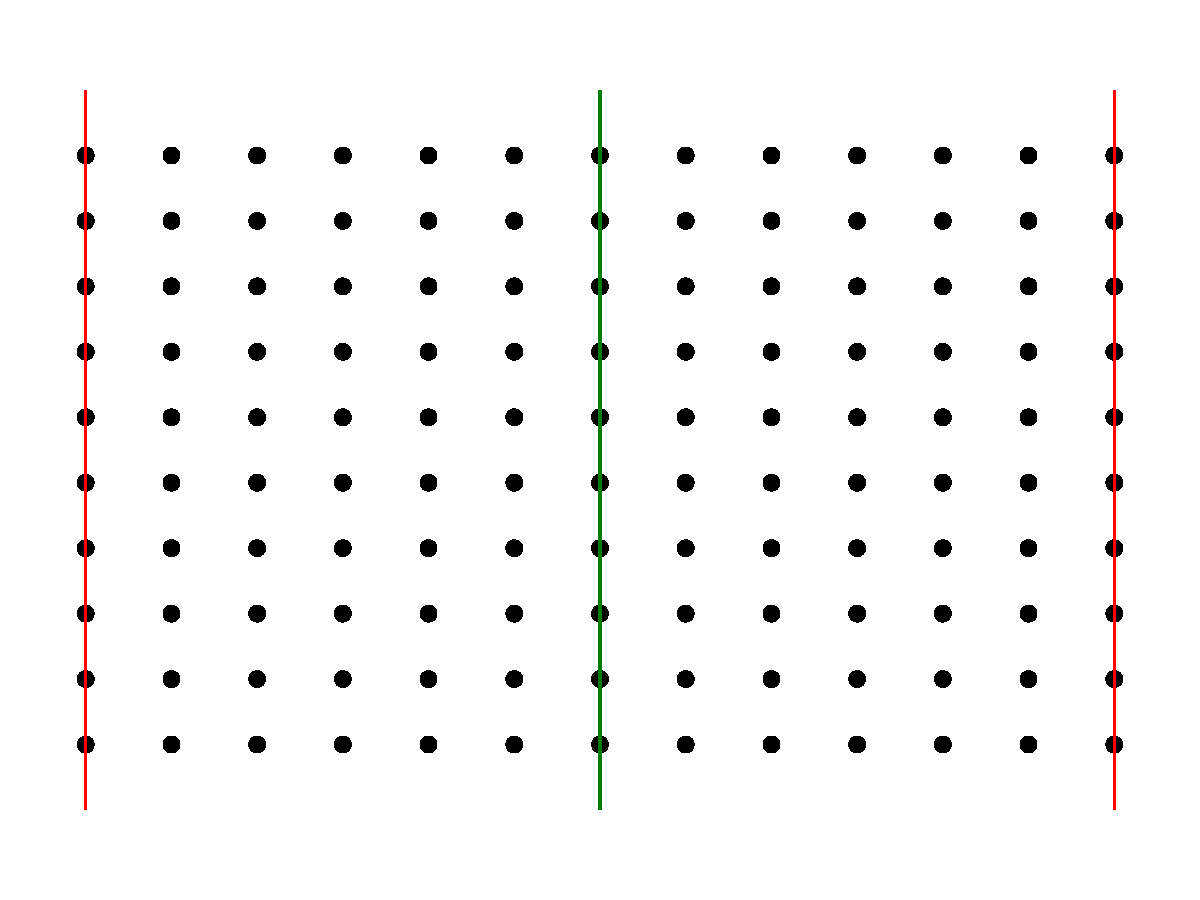
\includegraphics[width = \textwidth]{TMIntuition_1.pdf}
		\caption{\label{fig:TMIntuitionBare}}
	\end{subfigure}
	\centering
	\begin{subfigure}[b]{0.45\textwidth}
		\centering
		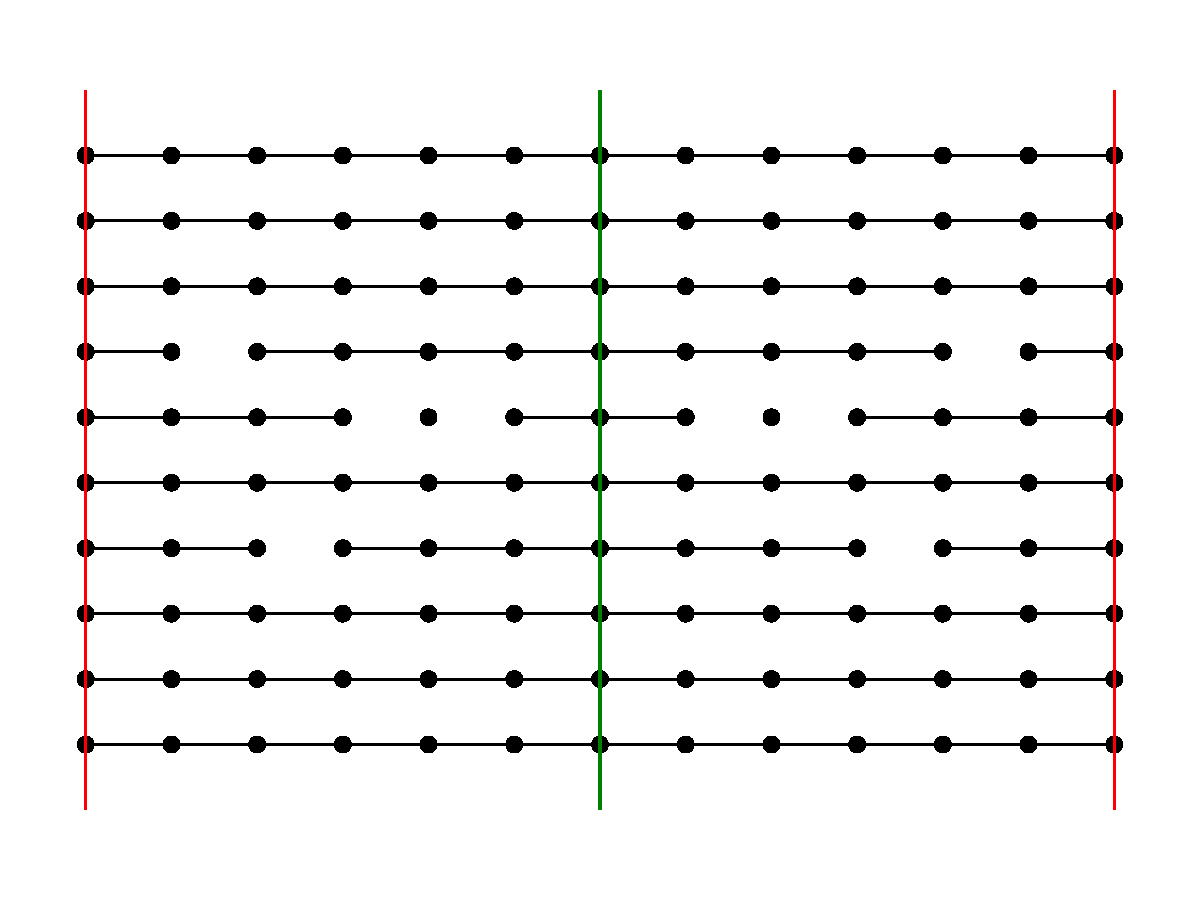
\includegraphics[width = \textwidth]{TMIntuition_2.pdf}
		\caption{\label{fig:TMIntuitionInherent}}
	\end{subfigure}
	\centering
	\begin{subfigure}[b]{0.45\textwidth}
		\centering
		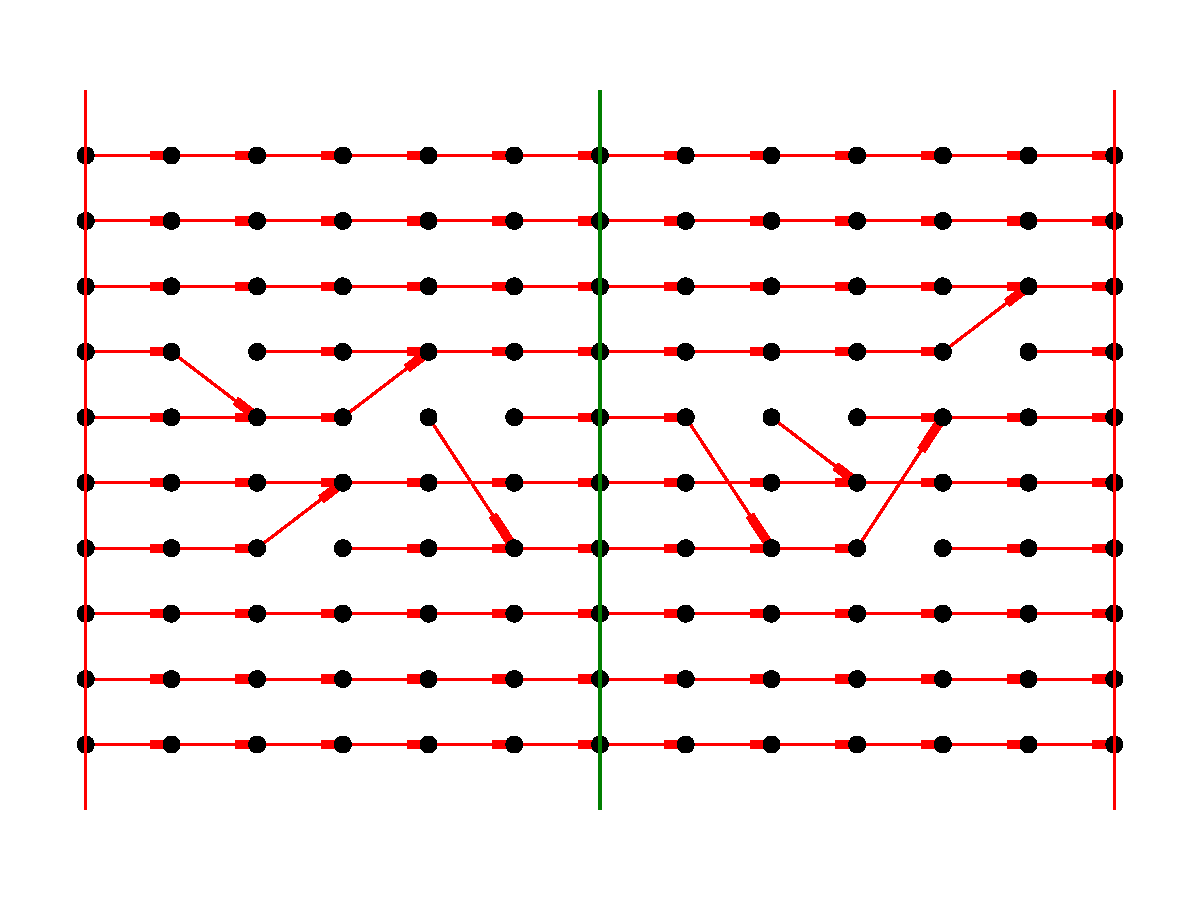
\includegraphics[width = \textwidth]{TMIntuition_3.pdf}
		\caption{\label{fig:TMIntuitionAQS}}
	\end{subfigure}
	\begin{subfigure}[b]{0.45\textwidth}
		\centering
		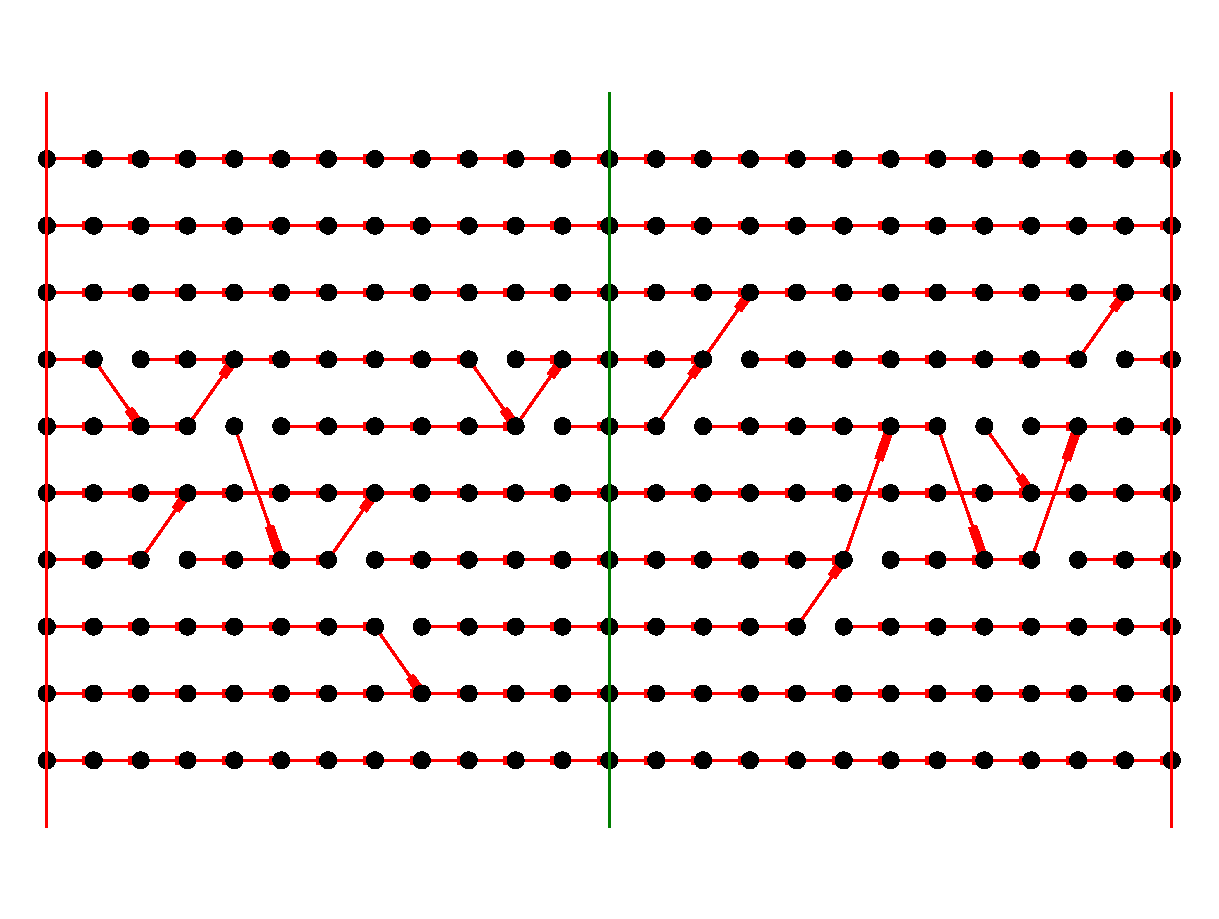
\includegraphics[width = \textwidth]{TMIntuition_4.pdf}
		\caption{\label{fig:TMIntuitionAQSMore}}
	\end{subfigure} 	
\caption{Diagrams exemplifying the assumptions of the TM model. It can be seen as a even more stripped down version of \autoref{fig:LifeOfInherentStructures}. In (\subref{fig:TMIntuitionBare}), just the minima of the energy landscapes associated to different values of $\gamma$ are plotted as black dots, with structures in the same landscape aligned on the same vertical line as $\gamma_{acc}$ is increased. The red lines represent the $\gamma = 0$ energy landscape, and the green one the $\gamma = \gamma_{max}$ landscape. In (\subref{fig:TMIntuitionInherent}), minima that continuously transform into each other as $\gamma_{acc}$ is changed are connected by black segments. If a structure is destroyed, it has no connection to any inherent structure on its right, whereas if an inherent structure is created, it is not connected to any minimum on its left. In (\subref{fig:TMIntuitionAQS}), the AQS dynamics of the systems moving from inherent structure to inherent structure is represented by red arrows. Whenever an inherent structure is destroyed, systems choose randomly a new inherent structure, accordingly to the assumptions of the TM model. The result is a directed graph that can be used to construct the $P_{+}$ and $P_{-}$ matrices associated to $\gamma_{max}$. In (\subref{fig:TMIntuitionAQSMore}), the same construction is applied for a different (larger) value of $\gamma_{max}$, obtaining a graph which extends the one in (\subref{fig:TMIntuitionAQS}) and has additional nodes in correspondence of the green line. \label{fig:TMIntuition}}
\end{figure}

\begin{figure}
\centering 
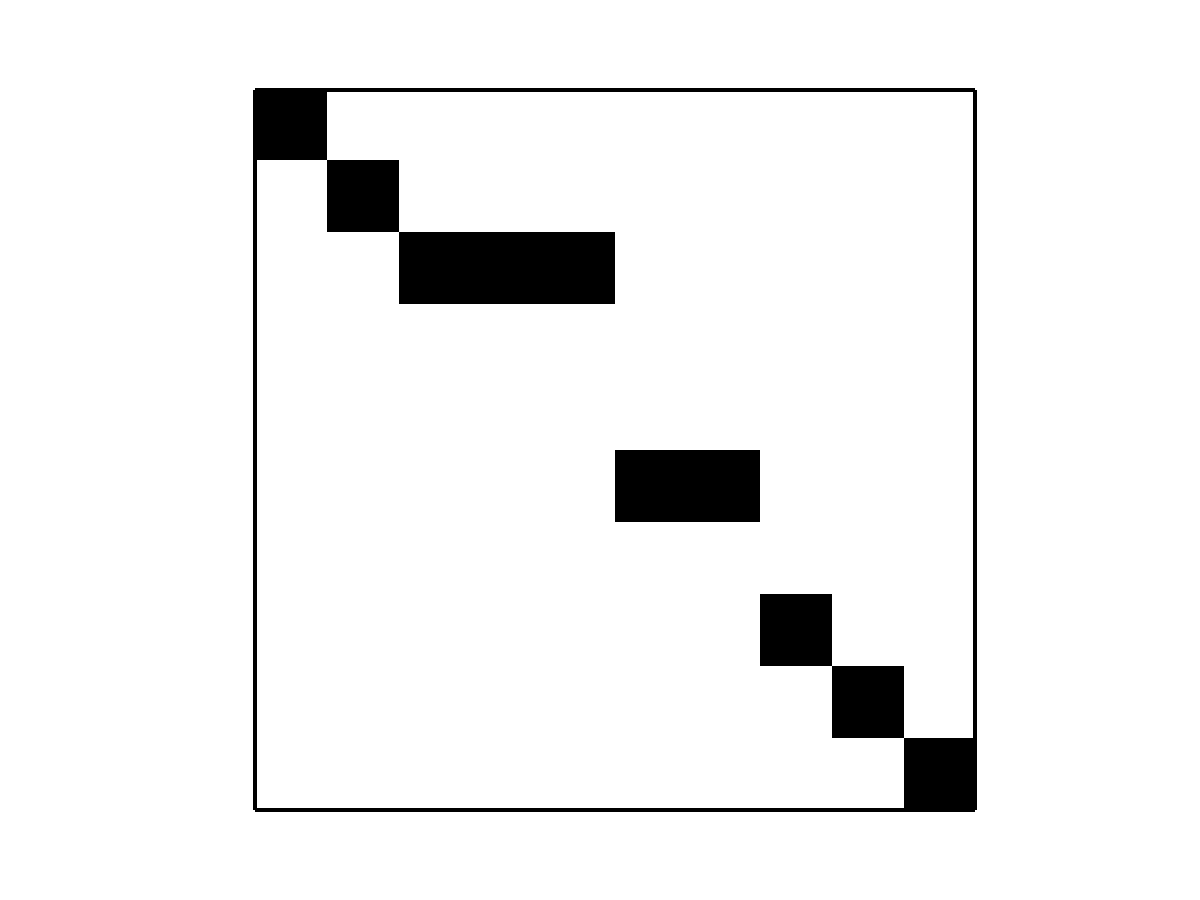
\includegraphics[width=0.48\textwidth]{TMIntuitionMatrix.pdf} 
\caption{Matrix $P_{+}$ summarizing the correspondences between the inherent structures in the graph in the directed graph in \autoref{fig:TMIntuitionAQS} representing AQS dynamics. A black (or white) square at position $(i,j)$ means that the entry at that position is one (or zero). A square at the position $(i,j)$ is black if the inherent structure $j$ maps into the structure $i$ through the AQS cycle represented in \autoref{fig:TMIntuitionAQS}.\label{fig:TMIntuitionMatrix}}
\end{figure}

\pagebreak

\section{Results from the NK model}
The NK and the LJ models share enough similarities so that one can perform on the former measurements that mirror those that have been performed on the latter in \autoref{ch:ParticleModelsResults}. In particular, the NK model possesses a deformable but \emph{discrete} energy landscape, that can be deformed in an oscillatory way. In what follows we show that the ingredients that the NK model retains are sufficient to display (at least qualitatively) the behavior observed in binary LJ mixtures, and in particular the existence of an absorbing to diffusive behavior transition at $\gamma_{c}$. The study of the NK model is thus helpful to single out the features of the LJ model that lead to the transition.\\
Unless noted otherwise, results below are averaged over $\approx 200$ different instances of the couplings $a$, $b$ and $J$ in \autoref{eq:NKNeighbors} and \autoref{eq:NKCouplings}, and obtained with a C code written by the author (see \autoref{app:DataPreservation}).

\subsection{NK at equilibrium}

Before performing simulations of ``deformation'' on NK samples one needs configurations to start from.
As in the case of the LJ systems discussed in \autoref{ch:ParticleModelsResults}, one would like to start from sets of configurations that differ for some feature (like the average potential energy). In this way one can check how deformation affects the samples, and how it is capable of making them evolve in such a way to forget their initial state. The obvious choice is to choose inherent structures differing for their effective $T$, exactly as in the LJ case.
Similarly to what has been performed in the case of particle systems above, we obtain several equilibrated NK configurations at different $T$. We do this for several realizations of the couplings $a$, $b$ and $J$ by means of Monte Carlo sampling and find their inherent structures of effective temperature $T$ by means of steepest descent (SD). The average energy of such inherent structures is plotted in \autoref{fig:InherentUvsTNK}, showing a behavior similar to that observed in \autoref{fig:UvsT}.
\begin{figure}[!h] 
\centering 
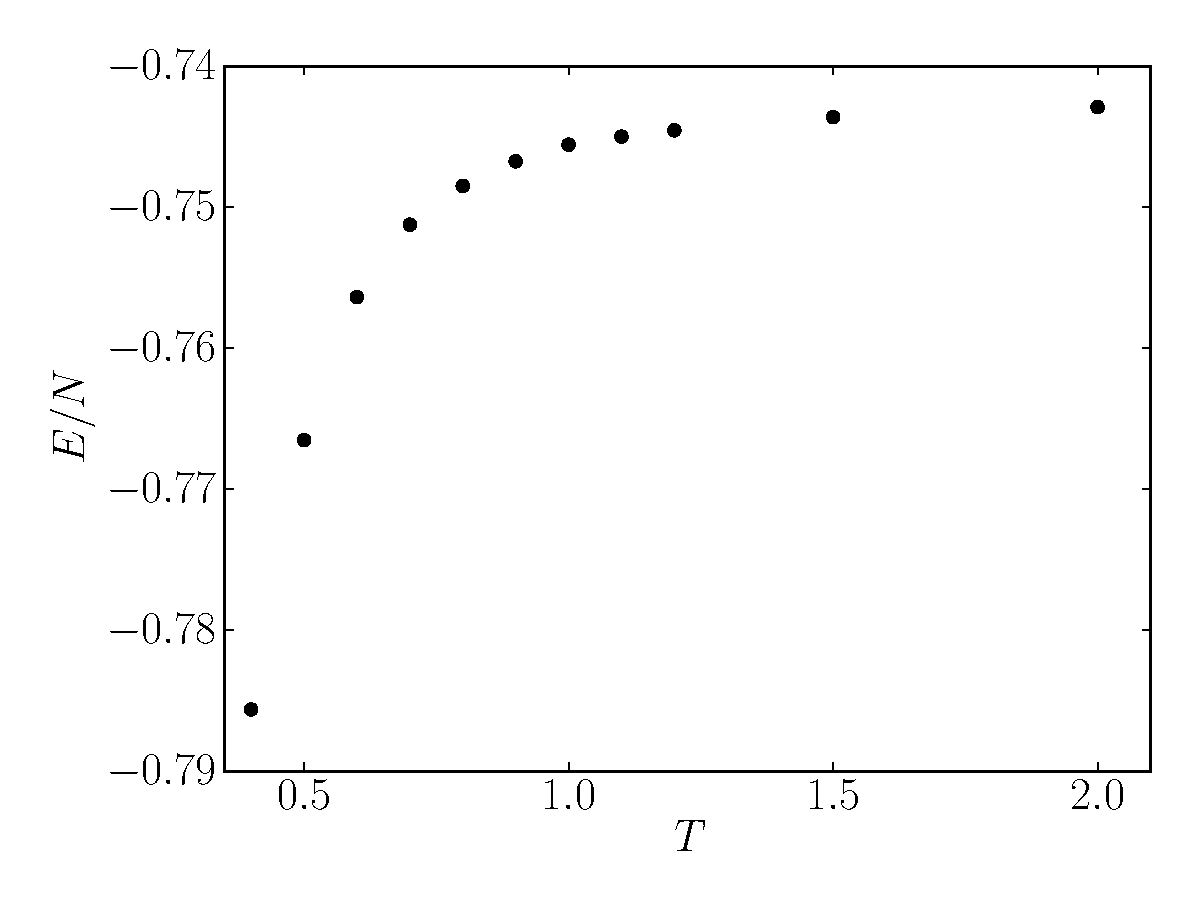
\includegraphics[width=0.8\textwidth]{EvsTNK20.pdf} 
\caption{Average energy per site of the inherent structures obtained by quenching NK samples ($N = 20$, $K=10$) equilibrated at different $T$. The plot bears a qualitative similarity with what is observed in particle models (see \autoref{fig:UvsT} for a comparison).\label{fig:InherentUvsTNK}}
\end{figure}
Even though the energy $U$ of inherent structures is expected to be a monotonically increasing function of $T$, the between \autoref{fig:InherentUvsTNK} and \autoref{fig:UvsT} is not entirely trivial, because it stems from the DOS of the inherent states and from the way in which inherent structures are connected with each other in the landscapes of the NK and KA models. Such analysis allows us to state that inherent structures at the effective temperatures $T = 0.6$ and $1.0$ are different enough to be distinguished. These values are thus selected as effective temperatures of choice for the initial inherent structures.

\subsection{Evolution of the energy under deformation}
We consider $N = 20, 40, 80$ and $K=10$, take $\approx 200$ instances of the couplings and obtain 3-4 equilibrated configurations at $T = 0.6$ and $1.0$ for each of such instances. The corresponding inherent structures obtained by SD are deformed by increasing $\gamma$ in \autoref{eq:NKEnergy} in steps of $d\gamma = 0.005$ (for all $N$) and performing SD at each step. The parameter $\gamma$ is varied in the interval $[-\gamma_{max}, \gamma_{max}]$ in a triangle wave fashion, exactly as in the AQS simulations seen in \autoref{ch:ParticleModelsResults}. The values of $E$ and the configuration are recorded whenever $\gamma = 0$, i.e. at intervals of $2\gamma_{max}$. Plots of $E$ as a function of $\gamma_{acc}$ (defined in the same way as in \autoref{eq:AccumulatedStrain}) are shown in \autoref{fig:UvsAccumulatedStrainNK} for the $N = 40$ case. Similarly to what is observed in the LJ case, for small values of $\gamma_{max}$ the energy reaches a plateau which depends on \emph{both} $\gamma_{max}$ and the initial effective $T$. For higher values of $\gamma_{max}$, all samples, regardless their initial effective $T$, reach plateau depending on $\gamma_{max}$ only. In this respect, the NK model is able to reproduce qualitatively the same behavior found in \autoref{fig:UvsAccumulatedStrainNK}, where samples forget about their initial preparation if the oscillation amplitude exceeds some value $\gamma_{c}$. Unlike the KA systems however, the NK model exhibits a peak in $E$ before the plateau, and thus can not be fit with a function of the form given in \autoref{eq:StretchedExponentialU}.

\begin{figure}
\centering 
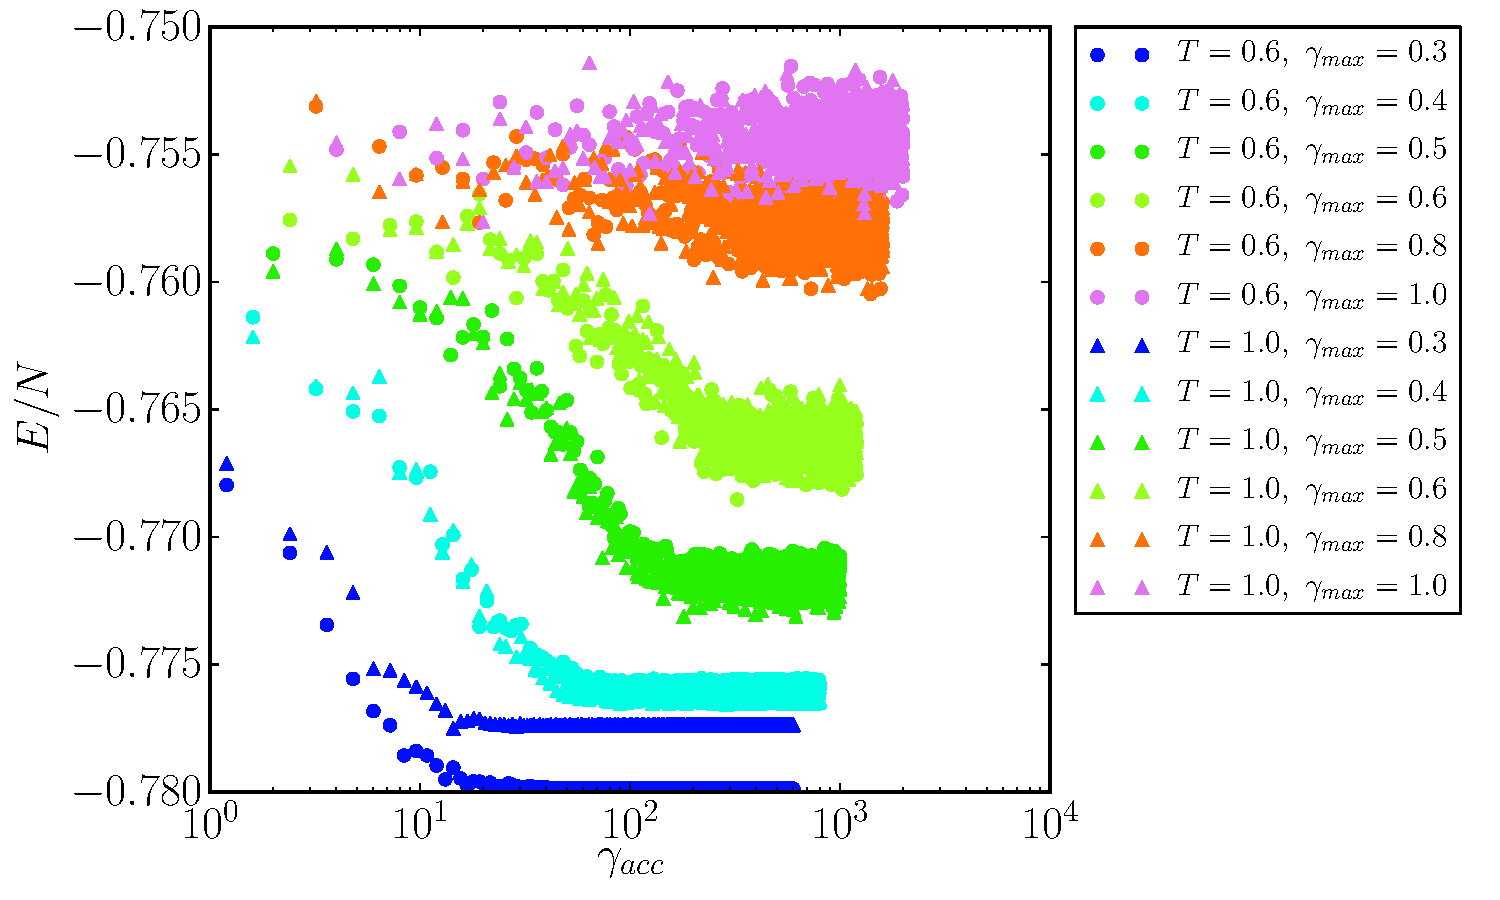
\includegraphics[width=0.8\textwidth]{ENK40.pdf} 
\caption{Potential energy per site as a function of $\gamma_{acc}$, for different initial effective temperatures and different deformation amplitudes $\gamma_{max}$, setting $N=40$, $K=10$. Data refer to configurations with $\gamma = 0$. For large values of $\gamma_{max}$ the energy fluctuates around some value which depends on $\gamma_{max}$ only. At small $\gamma_{max}$, instead, the plateau value of the energy depends on the effective $T$ of the initial configuration. In this respect what is observed here qualitatively resembles what has been found in particle models in \autoref{fig:UvsAccumulatedStrainKA}. \label{fig:UvsAccumulatedStrainNK}}
\end{figure}

\subsection{Diffusion behavior}

Changes in configurations under deformation can be studied for NK configuration as well, by looking at the distance between configurations before and after the application of deformation cycles.
Consider two configurations, $\mathbf{R}(\widetilde{\gamma}_{acc})$ and $\mathbf{R}(\gamma_{acc})$, obtained for values of the accumulated strain equal to $\widetilde{\gamma}_{acc}$ and $\gamma_{acc}$ respectively, with $\widetilde{\gamma}_{acc} < \gamma_{acc}$. Their distance can be expressed using the Hamming definition\footnote{In simpler terms, $d$ is the fraction of disagreeing components of the two vectors $\mathbf{r_{1}}$ and $\mathbf{r_{2}}$.} $d$:
\begin{equation}
	d(\gamma_{acc} - \widetilde{\gamma}_{acc}) = \frac{c_{01} + c_{10}}{N},
	\label{eq:HammingDistance}
\end{equation}
where $c_{01}$ ($c_{10}$) is the number of occurrences such that the $i$-th component of $\mathbf{R}(\widetilde{\gamma}_{acc})$ and the $i$-th component of $\mathbf{R}(\gamma_{acc})$ are respectively equal to 0 and 1 (to 1 and 0). 
We thus pick a configuration $\mathbf{r_{1}}$, choosing a large enough $\widetilde{\gamma}_{acc}$ so that the corresponding $E$ in \autoref{fig:UvsAccumulatedStrainNK} has relaxed to a steady state. We then compute the Hamming distance from it for configurations reached for increasing values of $\gamma_{acc}$, and plot it in \autoref{fig:HammingvsAccumulatedStrain}. Differently to what has been observed in \autoref{fig:MSDVsAccumulatedStrain}, samples don't show a diffusion behavior. In fact, the average Hamming distance measured starting from a reference configuration in the steady state quickly reaches a constant value for increasing $\gamma_{acc}$. This can be explained by the fact that when averaging the Hamming distance over many samples one is averaging over states that are absorbing (so that their Hamming distance is zero for any value of $\gamma_{acc}$) and others that quickly decorrelate from the reference state (so that the Hamming distance is 0.5). The observed value of the Hamming distance thus depends from the fraction of absorbing over non-absorbing states.\\
By plotting the average of such a value as a function of $\gamma_{max}$ for different values of $N$ (see \autoref{fig:AverageHammingvsGammaMax}), one observes that the capability of the system to move away from the reference configuration increases sharply at some value $\gamma_{c}$, which is roughly $N$ independent. The sharpness of the transition, moreover, is seen to increase with $N$. These data thus seem to confirm that a transition at some oscillation amplitude $\gamma_{c}$  from a localized regime to a diffusive one exists in the NK model, similarly to what is observed in our KA mixtures in \autoref{ch:ParticleModelsResults} and models of particle suspensions studied in \cite{keim2011generic} (see \autoref{sec:ShearedSuspensions}).

\begin{figure}
\centering 
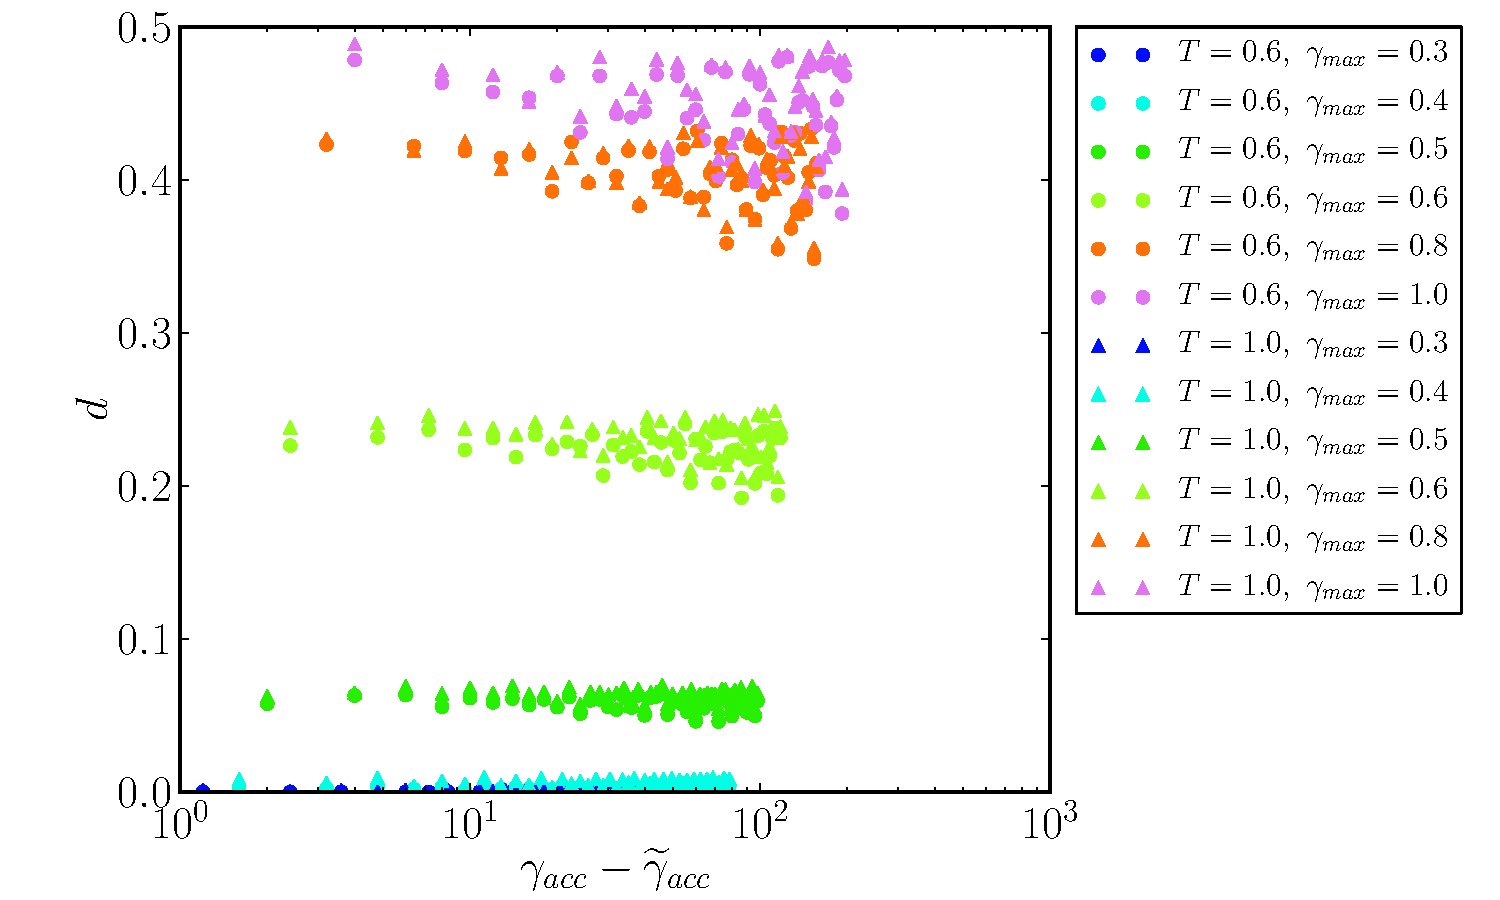
\includegraphics[width=0.8\textwidth]{HammingNK40.pdf} 
\caption{Hamming distance as a function of the accumulated strain measured from reference configurations with $\gamma_{acc} > \widetilde{\gamma}_{acc}$, where $\widetilde{\gamma}_{acc}$ marks the reaching of the plateau of the energy in \autoref{fig:UvsAccumulatedStrainNK}. $N=40$ and $K=10$. The behavior is not diffusive, but the higher the $\gamma_{max}$, the further the systems are able to move away from the reference configuration. The Hamming distance can be modeled with a constant function of $\gamma_{acc} - \widetilde{\gamma}_{acc}$. \label{fig:HammingvsAccumulatedStrain}}
\end{figure}

\begin{figure}
\centering 
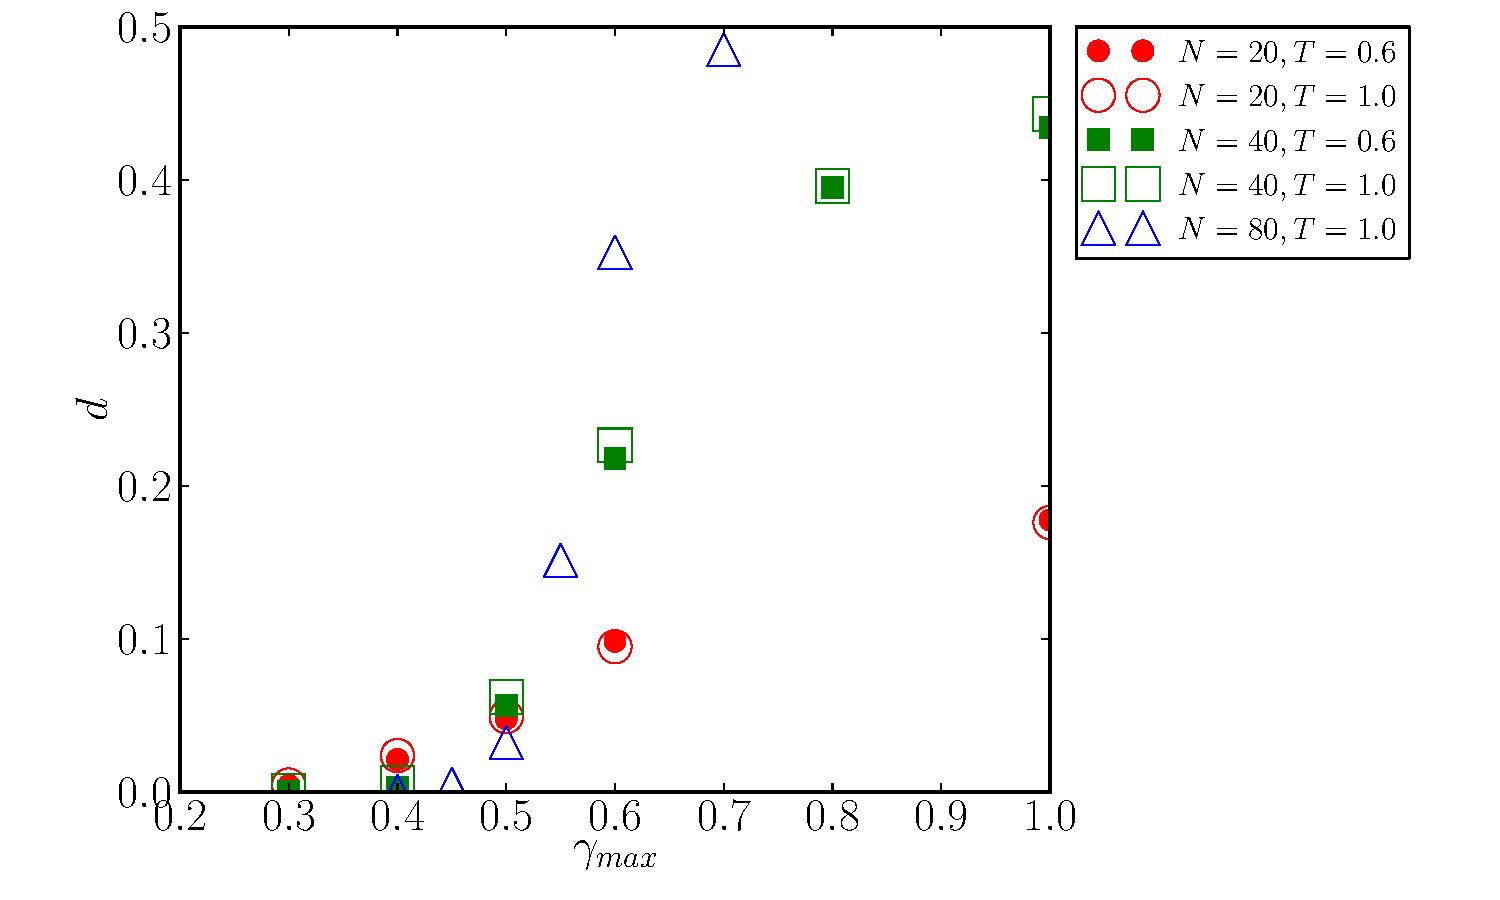
\includegraphics[width=0.8\textwidth]{AverageHamming.pdf} 
\caption{Average value of the Hamming distance as determined by averaging data like that in \autoref{fig:HammingvsAccumulatedStrain}, for different $N$ and setting $K=10$. The ability of the system to diffuse away from a reference configuration increases strongly with $\gamma_{max}$ at $\gamma_{max} \approx 0.5$. The transition become sharper as $N$ is increased. \label{fig:AverageHammingvsGammaMax}}
\end{figure}

\pagebreak

\section{Results from the TM model}

The TM model presented in \autoref{sec:TransitionMatrixModel} drops even more features of the LJ system with respect to the NK model: inherent configurations are not anymore associated to an energy, and there is no notion of topology and distance between them. The model consists of a highly stylized representation which mimics the evolution of inherent structures under oscillatory athermal deformation. In a nutshell, the model takes care of labeling all the inherent structures in a fictitious landscape at $\gamma = 0$ and determines a plausible form of the map $P$ that associates each inherent configuration with its image through a full deformation cycle (see discussion in \autoref{sec:TransitionMatrixModel}). Clearly, there is no possibility to straightforwardly\footnote{However, the TM model offers the possibility to extract a ``relaxation strain'' by looking at the average number of cycles $\widetilde{L}$ needed to the system to relax to an absorbing or recurring state (see discussion in \autoref{sec:TMStateClassification}). However, this possibility hasn't been explored in this work.} extract quantities like $\widetilde{\gamma}_{acc}$ and a diffusion constant within such a model.
The information contained in $P$ can be used to distinguish states that are absorbing or mapping to absorbing states from those that are recurring or mapping to recurring ones (see the definitions given in \autoref{sec:TMStateClassification}). This information, in turn, can be used to gather information about the dynamics under AQS deformation: if absorbing states dominate, systems are likely to be trapped into them, similarly to what is observed in the LJ and NK models below $\gamma_{c}$; if recurring states dominate, systems have the capability of exploring the configuration space before returning to the same state point, analogously to what happens in the other models above $\gamma_{c}$.

\subsection{``Diffusion'' behavior: absorbing and recurring states}

The naive way to determine which structures behave how under oscillatory deformation is to apply $P$ repeatedly to each of them. After some applications of $P$, the structures will transform into states of the kind $\mathbf{R_{abs}}$ such that $P \mathbf{R_{abs}} = \mathbf{R_{abs}}$ (absorbing), or states of the kind $\mathbf{R_{rec}}$ such that $P^{L} \mathbf{R_{rec}} = \mathbf{R_{rec}}$ (recurring). This procedure is however too expensive, because one needs to calculate the trajectory of each and every of the $M$ structures by means of matrix multiplication. 
A way to overcome this is treating $P$ as an adjacency matrix, and constructing the directed graph\footnote{A useful reference for the terminology of graph theory used in this paragraph is \cite{bollobas1998modern}.} $G$ associated to it (see \autoref{fig:DirectedGraphFromP}). $G$ will be a directed graph whose outdegree is 1, as each structure maps onto one and only one configuration through $P$. In general, $G$ will possess several connected components\footnote{Using the terminology of graph theory, $G$ is a \emph{directed 1-forest} or a \emph{functional graph} and its connected components are called 1-trees \cite{bollobas1998modern}.}. Each of these either contains a self-loop or not. Connected components containing a self-loop are those that contain an absorbing state, which is the very node that is connected to itself via the self-loop. All the other nodes are connected to it, and thus represent states mapping to the absorbing state. Connected components not containing self-loops must contain a loop, and their nodes thus represent recurring states or states mapping to recurring states. By examining the graphs one can count the number of $R$ of recurring (and mapping to recurring) states simply by counting the number of nodes of the connected components of $G$ which do not possess self-loops. The number of absorbing (and mapping to absorbing) states will be given by $M-R$.

\begin{figure}
	\centering
	\begin{subfigure}[b]{0.8\textwidth}
			\centering
			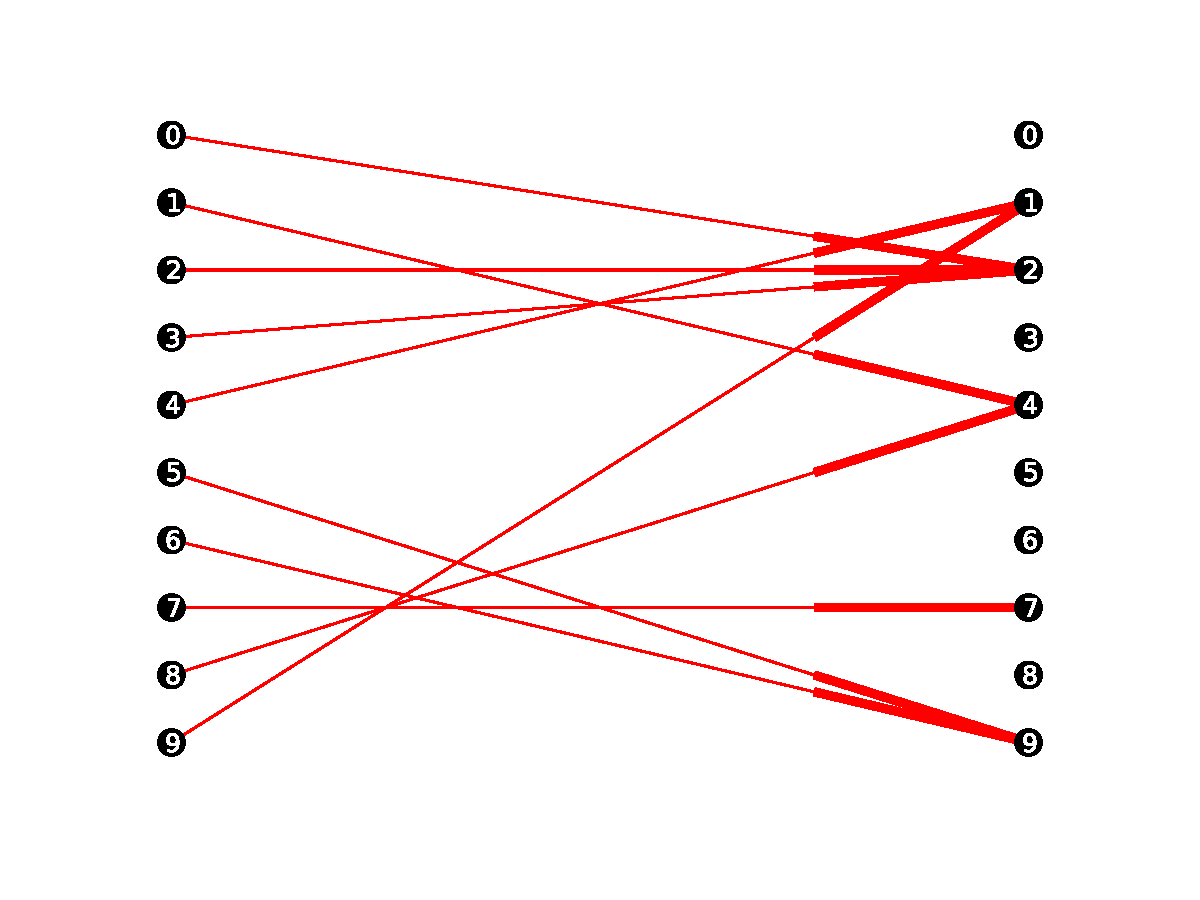
\includegraphics[width = 0.8\textwidth]{AQSMap1Forest.pdf}
			\caption{\label{fig:TMEndomorphism}}
	\end{subfigure}
	\begin{subfigure}[b]{0.8\textwidth}
			\centering
			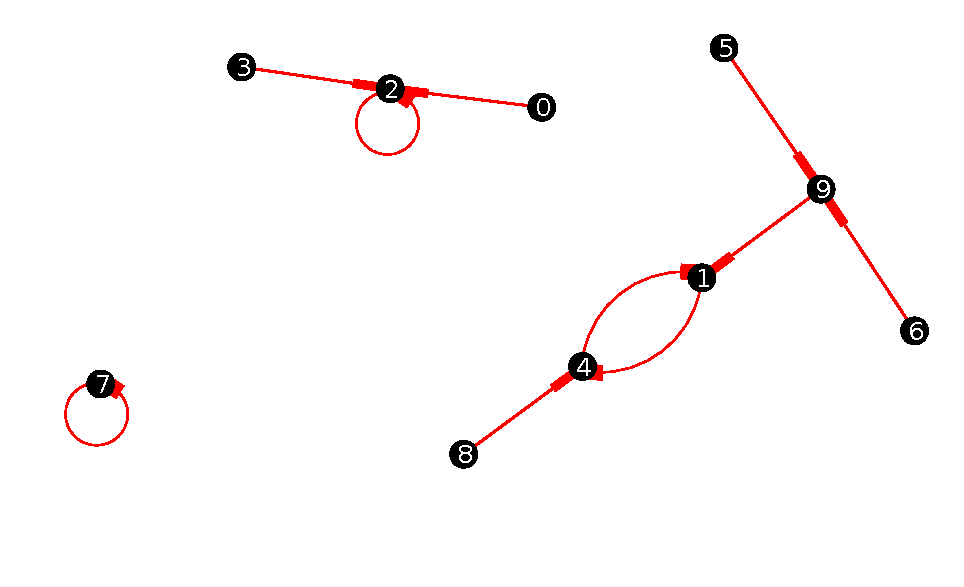
\includegraphics[width = 0.8\textwidth]{1Forest.pdf}
			\caption{\label{fig:TM1Forest}}
	\end{subfigure}
	\caption{(\subref{fig:TMEndomorphism}) The output of the TM model is a map (which depends on $\gamma_{max}$) of the set of inherent structures onto itself. The same map can be interpreted as an adjacency matrix for a directed graph. (\subref{fig:TM1Forest}) The resulting graph is a collection of 1-trees \cite{bollobas1998modern}. Each of these 1-trees can contain a self-loop or not. If it does, then the vertex with the self-loop represents an absorbing state, and all the vertices in the 1-tree to which it belongs represent states mapping to that absorbing state via AQS dynamics. If the 1-tree does not contain self-loops, then its vertices are associated either to recurring states or states that map onto recurring states in the AQS dynamics. By counting the number of vertices in the two kinds of 1-trees (those with self-loops and those without), one can thus determine the fraction of states that are absorbing (and mapping to absorbing) or recurring (and mapping to recurring).\label{fig:DirectedGraphFromP}}
\end{figure}

We obtain $P$ with the procedure described in \autoref{app:TMDetails}, using Python and the support for sparse matrices within the library SciPy \cite{scipy}. We then extract $G$ and its connected components using NetworkX \cite{networkx}. The connected components associated to recurring states can be easily filtered because they don't contain self-loops. We do so for matrices $P$ with $M = 10^{4}$, $10^{5}$ and $10^{6}$, setting (tentatively) the probability for an inherent structure to be destabilized per unit strain to $\tau = 0.04$ and plot the average fraction of recurring (or mapping to recurring) states as a function of the $\gamma_{max}$ averaging on $\approx 800, 200, 50$ matrices respectively.
The result is shown in \autoref{fig:RecurrentStateFractionVsGammaMax}.  

\begin{figure} 
\centering 
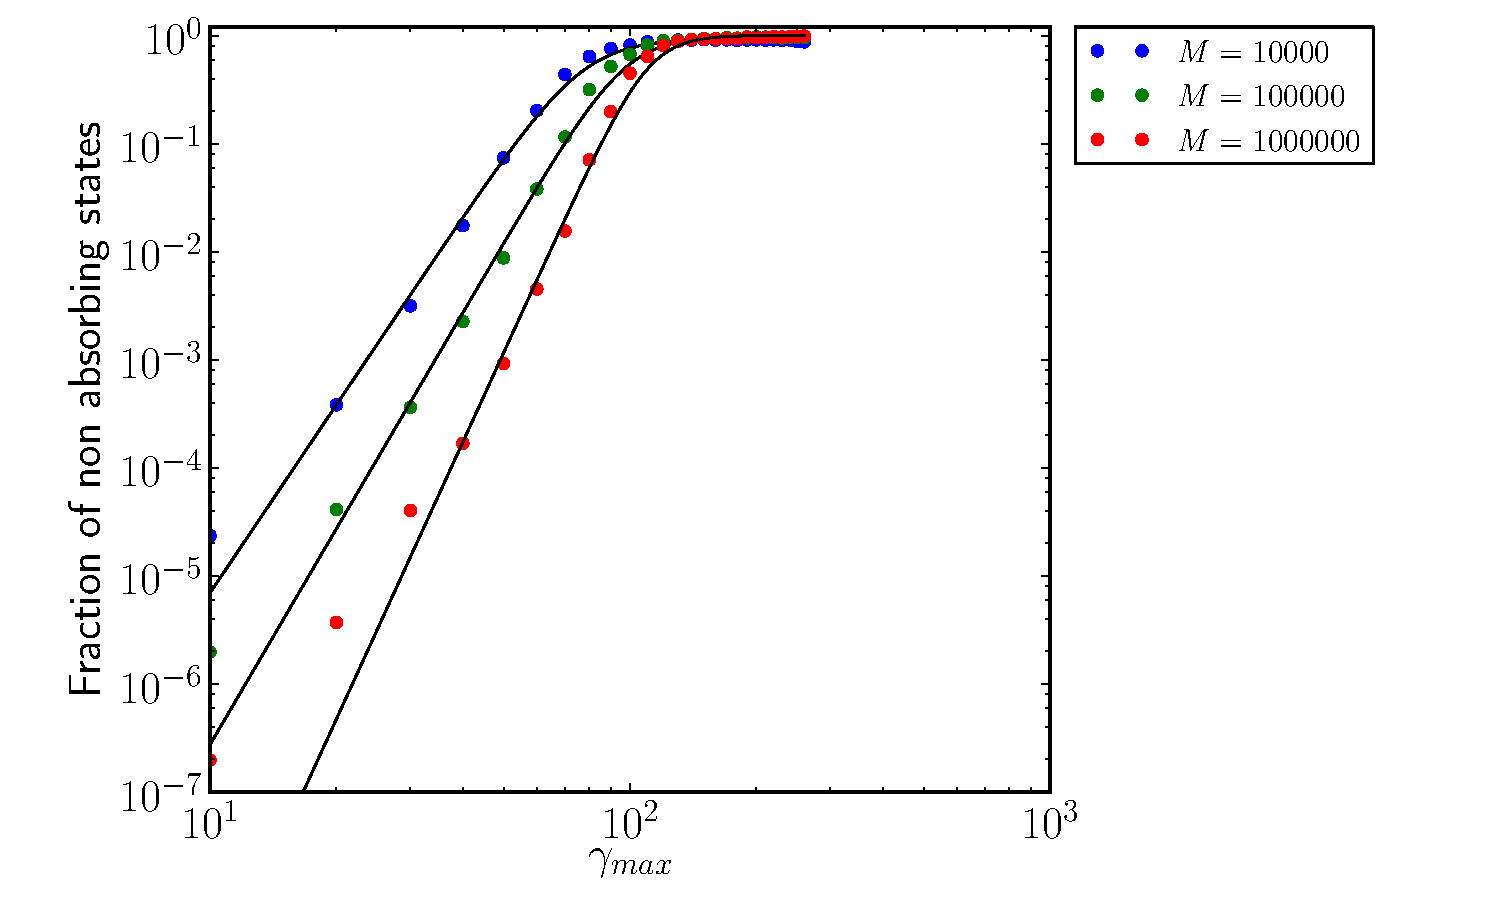
\includegraphics[width=0.8\textwidth]{RecurrentFractionTM.pdf} 
\caption{Overall fraction of recurring states and mapping to recurring states as a function of $\gamma_{max}$ for different values of $M$, obtained by analysis of the graphs associated to the transition matrices $P$ generated by the TM model. The number of recurring states increases strongly after some value $\gamma_{c}$ which increases as $M$ increases. The data can be described fairly well with the model in \autoref{eq:SaturatingPowerLaw} (black curves), with a sharpness (dictated by the parameter $a$) which increases for larger $M$. \label{fig:RecurrentStateFractionVsGammaMax}}
\end{figure}

The curves in \autoref{fig:RecurrentStateFractionVsGammaMax} can be modeled by the fitting function:
\begin{equation}
	f(x) = \frac{b}{1 + \left(\frac{\gamma_{c}}{\gamma_{max}} \right)^{a}}
	\label{eq:SaturatingPowerLaw}
\end{equation}

Data in \autoref{fig:RecurrentStateFractionVsGammaMax} and the form of \autoref{eq:SaturatingPowerLaw} show that the TM model shows a sharp increase in the number of states mapping to non-absorbing states as the ``oscillation amplitude'' is increased beyond some value $\gamma_{c}$, similarly to what has been observed in the case of LJ mixtures and of the NK model above. For this reason, one can reasonably believe that however crude, the TM model encapsulates enough details to describe qualitatively the switch from a ``localized'' regime (where absorbing states prevail) to a ``diffusive'' one (where recurring states dominate) observed in particle models. Moreover, the transition is observed to be sharper for higher values of $M$, with the parameter $a$ in \autoref{eq:SaturatingPowerLaw} increasing with increasing $M$. Opposite to what is observed in LJ systems, however, the value of $\gamma_{c}$ is seen to increase with the system ``size'' $M$.

\section{Summary}

In this chapter we have examined the behavior of two kinds of systems. \\
The first one is the NK model, which was already employed in the past \cite{isner2006generic} to determine if rejuvenation and overaging are phenomena which take place only in particle systems, or can occur in more general systems when they are cyclically driven in rugged landscapes.
The second is a ``transition matrix'' (TM) model that was specifically designed by us to rationalize the behavior of the dynamics of inherent structures of particle systems under oscillatory athermal deformation. \\
These systems show a behavior that has interesting similarities and differences with that of particle models studied in \autoref{ch:ParticleModelsResults}. \\
As for the NK model, it exhibits an energy behavior under oscillatory driving that is reminiscent of that observed in the LJ systems of \autoref{ch:ParticleModelsResults}. If samples are driven with an amplitude $\gamma_{max}$ above some threshold driving amplitude $\gamma_{c}$, the energy curves as a function of the accumulated ``strain'' $\gamma_{acc}$ do converge to a common value, regardless the initial value of the effective temperature (\autoref{fig:UvsAccumulatedStrainNK}). This doesn't happen below $\gamma_{c}$, as systems with different effective $T$ do reach different plateau values of the energy $E$ when they are driven at the same $\gamma_{max}$. However, we couldn't devise a way to describe $E$ as a function of $\gamma_{acc}$. In addition, the cumulative $\gamma_{acc}$ needed to reach the plateau doesn't seem to increase in correspondence of any value of $\gamma_{max}$, as opposed to what is observed in the LJ models. \\
As for the dynamics in configuration space, the NK model exhibits another important distinctive feature: it shows no hint of diffusion, as configurations seem to reach and mantain a steady average distance from a reference configuration as $\gamma_{acc}$ is increased (\autoref{fig:HammingvsAccumulatedStrain}). However, such distance increases with $\gamma_{max}$, and when plotted against $\gamma_{max}$ it shows a sigmoidal trend which increases at a value $\gamma_{c}$, with a sharpness depending on $N$ (\autoref{fig:AverageHammingvsGammaMax}). We thus posit that a transition at a value $\gamma_{c}$ holds for the NK model, even though our data are too scarce to model it. Our values of $N$ are quite small with respect to $K$, so our samples are possibly affected by important size effects. It would be interesting to study larger samples and do a proper analysis of size effects. Unfortunately, a study of the NK model becomes quickly prohibitive for large $N$. A possible solution would be parallelizing the NK code so to allow it to split the minimization procedure onto several processors, but such a scheme has not been implemented in this thesis.\\
We used the TM model to compute the fraction of states that map (via AQS dynamics) to recurring states as a function of $\gamma_{max}$. Recurring states are expected to represent the diffusive states encountered in the LJ model, at least in the limit in which the number of inherent structures $M$ is large. Indeed the fraction of recurring states and states mapping to recurring states grows with $\gamma_{max}$ (see \autoref{fig:RecurrentStateFractionVsGammaMax}) and it is well fitted by \autoref{eq:SaturatingPowerLaw}. Such fraction of recurring states is related to the observations of diffusion in the LJ model, but can't directly be compared with it, because there is no notion of spatial distance in the TM model. However, such result is in qualitative agreement with what is observed in both the NK and LJ models, showing that the TM model is able to qualitatively capture their behavior.

